\documentclass[12pt,oneside]{book}

\usepackage[english]{babel}
\usepackage[utf8]{inputenc}  
\usepackage[T1]{fontenc}
\usepackage{listings}
\usepackage{comment}
\usepackage[left=2.5cm,right=2.5cm,top=3cm,bottom=2.65cm]{geometry}
\usepackage{graphicx}
\usepackage{tabularx}
\usepackage{amsmath,amssymb,amsfonts}
\usepackage{bbm, bm}
\usepackage{stmaryrd}
\usepackage{mathtools}
\usepackage{hyperref}
\usepackage{tikz}
\usepackage{tabularx}
\usepackage{makecell}
\usepackage{color}
\usepackage{fancybox}
\usepackage[thmmarks,amsmath]{ntheorem}
\usepackage{minitoc}
\usepackage{titletoc}
\usepackage{algpseudocode}
\usepackage[ruled,vlined]{algorithm2e}
\usepackage{wrapfig}
\usepackage{kpfonts}
\usepackage{capt-of}
\usepackage{caption}
\usepackage{tikz}

\graphicspath{{ims/}}

\DeclareMathOperator*{\argmax}{arg\,max}
\DeclareMathOperator*{\argmin}{arg\,min}

\usetikzlibrary{arrows.meta}
\usetikzlibrary{arrows}
\usetikzlibrary{decorations.pathreplacing}
\usetikzlibrary{intersections}

\mathtoolsset{showonlyrefs=true}

\addto\extrasenglish{%
	\def\subsectionautorefname{\S}%
	\def\sectionautorefname{\S}%
}

\definecolor{darkWhite}{rgb}{0.94,0.94,0.94}
\definecolor{blue}{rgb}{0.12,0.16,0.53}
\definecolor{green}{rgb}{0.25,0.28,0.06}
\definecolor{purple}{rgb}{0.5, 0.1, 0.5}
\definecolor{yellow}{rgb}{0.8, 0.7, 0.1}
\definecolor{greenTikz}{rgb}{0.16,0.53,0.12}
\definecolor{red}{rgb}{0.71,0.19,0.11}
\definecolor{redLight}{rgb}{0.85,0.24,0.15}
\definecolor{darkPurple}{rgb}{0.2,0.05,0.18}
\definecolor{whiteGray}{rgb}{0.92,0.96,0.95}

\newcounter{sss}[subsection]
\renewcommand\thesection{\textcolor{red}{\Roman{section} -}}
\renewcommand\thesubsection{\textcolor{blue}{\arabic{subsection}/}}
\renewcommand\thesss{\textcolor{green}{\alph{sss}.}}
\renewcommand\thechapter{\Alph{chapter}}
\newcommand{\sect}[1]{\section{\textcolor{red}{#1}}}
\newcommand{\subs}[1]{\subsection{\textcolor{blue}{#1}}}
\newcommand{\subsubs}[1]{
	\stepcounter{sss}
	\subsubsection{\textcolor{green}{\thesss~#1}}
}

\newcommand{\mybox}[4]{
	\begin{center}
		\boxput*(0,1){\colorbox{darkWhite}{\textbf{#1}}}{
			\setlength{\fboxsep}{12pt}
			\fcolorbox{#2}{#3}{
				\begin{Bflushleft}
					\begin{minipage}{0.908\linewidth}
						\vspace{2mm} \par \textcolor{#2}{#4}
					\end{minipage}
				\end{Bflushleft}
			}
		}
	\end{center}
}

\newcommand{\mytitle}[1]{
	\title{
		\fcolorbox{black}{whiteGray}{
			\begin{Bflushleft}
				\\ \huge \textbf{\textcolor{red}{#1}}
			\end{Bflushleft}
		}
	}
}

\setcounter{tocdepth}{1}
\setcounter{minitocdepth}{3}
\nomtcrule
\titlecontents*{chapter}[0pt]{}
{\bfseries\chaptername\ \thecontentslabel\quad}{}
{\bfseries\hfill\contentspage}
\newcommand{\mytoc}{
	\renewcommand{\contentsname}{}
	\mybox{Table des matières}{darkPurple}{darkWhite}{
		\vspace{-40mm}\tableofcontents}
}
\newcommand{\myminitoc}{
	\mybox{Table des matières}{darkPurple}{darkWhite}{
		\vspace{-9mm}\minitoc \vspace{-8mm}}
}


\newcommand{\DEF}[1]{\vspace{1mm} \mybox{Definition}{blue}{white}{#1}}
\newcommand{\REM}[1]{\vspace{1mm} \mybox{Remark}{darkPurple}{white}{#1}}

\newcounter{propNum}
\newcommand{\PROP}[2][]{
	\stepcounter{propNum}
	\vspace{1mm}
	\mybox{Proposition \thepropNum #1}{red}{white}{#2}
}
\newcommand{\dem}{\paragraph{Demonstration}}
\newcommand{\findem}{\hfill $\blacksquare$}
\newcommand{\exe}{\paragraph{\textit{\textcolor{green}{Exemple}}}}

\newcommand{\N}{\mathbf{N}}
\newcommand{\trans}{\mathsf{T}}
\newcommand{\R}{\mathbf{R}}
\newcommand{\Pp}{\mathbb{P}}
\newcommand{\E}{\mathbb{E}}
\newcommand{\X}{\mathcal{X}}
\newcommand{\Y}{\mathcal{Y}}
\newcommand{\Z}{\mathcal{Z}}
\newcommand{\dist}{\mathcal{D_Z}}
\newcommand{\Hyp}{\mathcal{H}}
\newcommand{\trisk}{\mathcal{R}^l}
\newcommand{\erisk}{\hat{\mathcal{R}}^l}
\newcommand{\vrisk}{\tilde{\mathcal{R}}}

\mytitle{Optimal Transport in Machine Learning}
\author{
	Yoann Coudert--Osmont
	\and
	Nemo Fournier
}
\date\today

\begin{document}
	
	\dominitoc[n]
	\maketitle
	\mytoc
	
	\chapter{Overview of Optimal Transport}

\myminitoc

Optimal transport aims to define a geometry and a distance on the set of
mesures of probability on a space.

\sect{Introduction}

\subs{\textsc{Monge}'s Problem}

\begin{center}
	\begin{tikzpicture}[>=stealth']
		\draw[fill=brown!20] (-1, -1.8) rectangle (9, 0);
		\draw[fill=red, domain=0:2, smooth, variable=\x, fill opacity=0.9]
			plot({1.5*\x}, {\x * (27.21 + \x * (-126.6 + \x * (229.9 + \x * (-200.7
				+ \x * (84.24 - 13.61 * \x)))))}) -- (3.05, 0);
		\node[red] at (-0.2, 0.7) {$\mu$};
		\draw[fill=blue, fill opacity=0.9]
			(5, 0) -- (5.1, -1.2) -- (5.5, -1.2) -- (5.6, -1) -- (5.9, -1) --
			(6, -1.2) -- (6.4, -1.2) -- (6.5, -1) -- (6.8, -1) -- (6.9, -1.2) --
			(7.3, -1.2) -- (7.4, -1) -- (7.7, -1) -- (7.8, 0);
		\node[blue] at (8, -1.2) {$\nu$};
		\draw[ultra thick, purple] (0.4, 0) -- (0.4, 1.68);
		\draw[ultra thick, purple] (6.1, 0) -- (6.1, -1.2);
		\node[red] (x) at (0.4, -0.15) {$\bullet$};
		\node[blue] (y) at (6.1, 0.15) {$\bullet$};
		\node[below] at (x) {$x$};
		\node[above] at (y) {$y = T(x)$};
		\coordinate (y) at (6, 0.1);
		\draw[->, ultra thick, greenTikz, bend right=30]
			(x) edge node[below, black] {${\color{greenTikz}c}(x, T(x))$} (y);
	\end{tikzpicture}
\end{center}

\paragraph{Monge}

We work on a space of probability $\Omega$. We consider two mesures of
probability $\mu$ and $\nu$ on $\mathcal{P}(\Omega)$. We also consider a cost function
$c : \Omega \times \Omega \rightarrow \R$. This function can for instance be the Euclidean distance. Monge's problem is therefore the following

$$ \int_{\Omega} c \left( x, T(x) \right) \mu(x) $$
\vspace{-2mm}
$$ \text{s.t.} \quad \forall A \in \mathcal{P}(\Omega), \, \nu(A) = \mu \left( T^{-1}(A) \right) $$

The function $T$ is called a transport map. It carries the information
regarding the displacement of each elementary unit of probability: the mass
located in $x$ is moved toward $T(x)$. The function $c$ thus allows to
quantify the cost of the displacement of one elementary unit of mass. We
want to minimize the average distance travelled by mass units during the
optimal transport.

\paragraph{Limitations}

The issue with this formulation of an optimal transport problem is that it
doesn't handle discrete probability mesures. Indeed, if $\mu$ has a Dirac
impulse bigger than every Dirac impulse of $\nu$, then the transport map
cannot be build.

\subs{Kantorovich's problem}

\begin{center}
	\begin{tikzpicture}[>={latex}, scale=1.2]
		\draw[->, greenTikz, ultra thick] (5.20, 3.65) -- node[black, above] {60} (3.96, 3.47);
		\fill[red] (5.20, 3.65) circle (0.136) node[white] {\tiny 60};
		\fill[blue] (3.65, 3.42) circle (0.313) node[white] {120};
		\draw[->, greenTikz, ultra thick] (6.69, 0.87) -- node[black, above right] {90} (5.21, 1.91);
		\fill[red] (6.69, 0.87) circle (0.221) node[white] {90};
		\fill[blue] (0.33, 0.18) circle (0.221) node[white] {90};
		\draw[->, greenTikz, ultra thick] (3.73, 0.65) -- node[black, left] {60} (3.66, 3.11);
		\draw[->, greenTikz, ultra thick] (3.73, 0.65) -- node[black, above] {90} (0.55, 0.21);
		\fill[red] (3.73, 0.65) circle (0.409) node[white] {150};
		\fill[blue] (5.03, 2.04) circle (0.221) node[white] {90};
		
		\node[red, below] at (5.2, 3.55) {\textbf{1}};
		\node[red, right=6] at (6.69, 0.87) {\textbf{2}};
		\node[red, below right=9] at (3.73, 0.65) {\textbf{3}};
		\node[blue, left=8] at (3.65, 3.42) {\textbf{A}};
		\node[blue, left=6] at (0.33, 0.18) {\textbf{B}};
		\node[blue, above=6] at (5.03, 2.04) {\textbf{C}};
	\end{tikzpicture}
\end{center}

\paragraph{Changement de plan de transport}
\paragraph{Change of transport plan}
The idea of Kantorovich is to change the function $T : \Omega \rightarrow
\Omega$ into a probability $P$ on the product space $\mathcal{P}(\Omega \times
\Omega)$. On the upper example, Monge's formulation forbids to separate the
masse of size 150 into two separate masses. With Kantorovich's formulation,
this operation is accessible: the mass of $150$ is splitted into a mass of
$90$ and a mass of $60$, both sent to different places. In the discrete
case, we can represent what happens with a matrix.

\begin{center}
	\begin{tikzpicture}
		\draw[step=1, thick] (0, 0) grid (3, 3);
		\node at (0.5, 0.5) {\Large $p_{{\color{red}3}{\color{blue}A}}$};
		\node at (1.5, 0.5) {\Large $p_{{\color{red}3}{\color{blue}B}}$};
		\node at (2.5, 0.5) {\Large $p_{{\color{red}3}{\color{blue}C}}$};
		\node at (0.5, 1.5) {\Large $p_{{\color{red}2}{\color{blue}A}}$};
		\node at (1.5, 1.5) {\Large $p_{{\color{red}2}{\color{blue}B}}$};
		\node at (2.5, 1.5) {\Large $p_{{\color{red}2}{\color{blue}C}}$};
		\node at (0.5, 2.5) {\Large $p_{{\color{red}1}{\color{blue}A}}$};
		\node at (1.5, 2.5) {\Large $p_{{\color{red}1}{\color{blue}B}}$};
		\node at (2.5, 2.5) {\Large $p_{{\color{red}1}{\color{blue}C}}$};
		
		\node at (1.5, 3.5) {\large Transport Map};
		\node[blue] at (0.5, -0.5) {\Large 120};
		\node[blue] at (1.5, -0.5) {\Large 90};
		\node[blue] at (2.5, -0.5) {\Large 90};
		\node[red] at (-0.5, 0.5) {\Large 60};
		\node[red] at (-0.5, 1.5) {\Large 90};
		\node[red] at (-0.5, 2.5) {\Large 150};
		
		\node at (7.5, 3.5) {\large Distance matrix};
		\draw[step=1, thick] (6, 0) grid (9, 3);
		\node at (6.5, 0.5) {\Large $d_{{\color{red}3}{\color{blue}A}}$};
		\node at (7.5, 0.5) {\Large $d_{{\color{red}3}{\color{blue}B}}$};
		\node at (8.5, 0.5) {\Large $d_{{\color{red}3}{\color{blue}C}}$};
		\node at (6.5, 1.5) {\Large $d_{{\color{red}2}{\color{blue}A}}$};
		\node at (7.5, 1.5) {\Large $d_{{\color{red}2}{\color{blue}B}}$};
		\node at (8.5, 1.5) {\Large $d_{{\color{red}2}{\color{blue}C}}$};
		\node at (6.5, 2.5) {\Large $d_{{\color{red}1}{\color{blue}A}}$};
		\node at (7.5, 2.5) {\Large $d_{{\color{red}1}{\color{blue}B}}$};
		\node at (8.5, 2.5) {\Large $d_{{\color{red}1}{\color{blue}C}}$};
	\end{tikzpicture}
\end{center}

\paragraph{Discrete Case}

If we note $D$ our disance matrix, we obtain the following formulation in the discrete case:

$$ \min_P \langle P, D \rangle = \sum_i \sum_j p_{ij} d_{ij} $$
\vspace{-4mm}
$$ \text{s.t.} \quad \left\{ \begin{array}{ll}
\forall i & \sum_j p_{ij} = \mu_i \\
\forall j & \sum_i p_{ij} = \nu_j
\end{array} \right. $$

\paragraph{Continuous Case}

In the continuous setting, we introduce the following set of joint probabilities:

$$ \Pi(\mu, \nu) = \left\{ P \in \mathcal{P}(\Omega \times \Omega)~|~\forall A, B \in \Omega, \, P(A \times \Omega) = \mu(A), \, P(\Omega \times B) = \nu(B) \right\} $$

This set encodes the conditions of the discrete case but in the very
continuous setting. We consider once again our cost function $c$ defined
in the Monge's problem. Kantorovich's formulation now becomes the following
optimization problem:

$$ \inf_{P \in \Pi(\mu, \nu)} \E_P \left[ c(X, Y) \right] = \int \int c(x, y) P(dx, dy) $$
\subs{Wasserstein distance}

This optimization problem allows us to define a distance between probability mesures:

\DEF{
    Given a probability space $\Omega$, a cost function $c : \Omega \times
    \Omega \rightarrow \R$ and two probabilitiy mesures $\mu$ and $\nu$ in
    $\mathcal{P}(\Omega)$, the \textbf{p-Wasserstein-distance} between $\mu$
    and $\nu$ is defined by :
	$$ W_p(\mu, \nu) = \left( \inf_{P \in \Pi(\mu, \nu)} \int \int c(x,
	y)^p P(dx, dy) \right)^{1 / p} $$
	\vspace{-3mm}
}

This distance allows to compute barycenters between several probability
distributions, and obtain results that are way more natural than barycenters
obtained with other norms, like $l_2$ for instance. The following
figure compares an interpolation (progressive weighted barycenter of two
distributions) obtained via Wasserstein-distance and a linear interpolation.

\begin{center}
	\begin{tikzpicture}[scale=0.85]
		\node at (5.5, 4.5) {\large Interpolation linéaire};
		\node[red] at (0.5, 2.3) {$\mu$};
		\node[blue] at (9.5, 2.7) {$\nu$};
		\fill[red] (0.000, 0.000) -- (0.050, 0.403) -- (0.100, 0.752) -- (0.150, 1.051) -- (0.200, 1.302) -- (0.250, 1.509) -- (0.300, 1.676) -- (0.350, 1.806) -- (0.400, 1.902) -- (0.450, 1.967) -- (0.500, 2.004) -- (0.550, 2.016) -- (0.600, 2.006) -- (0.650, 1.976) -- (0.700, 1.929) -- (0.750, 1.868) -- (0.800, 1.794) -- (0.850, 1.710) -- (0.900, 1.618) -- (0.950, 1.521) -- (1.000, 1.419) -- (1.050, 1.315) -- (1.100, 1.211) -- (1.150, 1.108) -- (1.200, 1.008) -- (1.250, 0.912) -- (1.300, 0.822) -- (1.350, 0.738) -- (1.400, 0.662) -- (1.450, 0.595) -- (1.500, 0.537) -- (1.550, 0.490) -- (1.600, 0.455) -- (1.650, 0.431) -- (1.700, 0.419) -- (1.750, 0.420) -- (1.800, 0.435) -- (1.850, 0.462) -- (1.900, 0.503) -- (1.950, 0.556) -- (2.000, 0.623) -- (2.050, 0.703) -- (2.100, 0.796) -- (2.150, 0.900) -- (2.200, 1.017) -- (2.250, 1.144) -- (2.300, 1.281) -- (2.350, 1.428) -- (2.400, 1.584) -- (2.450, 1.746) -- (2.500, 1.915) -- (2.550, 2.089) -- (2.600, 2.267) -- (2.650, 2.447) -- (2.700, 2.627) -- (2.750, 2.807) -- (2.800, 2.984) -- (2.850, 3.156) -- (2.900, 3.321) -- (2.950, 3.478) -- (3.000, 3.624) -- (3.050, 3.757) -- (3.100, 3.874) -- (3.150, 3.973) -- (3.200, 4.052) -- (3.250, 4.107) -- (3.300, 4.136) -- (3.350, 4.137) -- (3.400, 4.105) -- (3.450, 4.038) -- (3.500, 3.933) -- (3.550, 3.787) -- (3.600, 3.595) -- (3.650, 3.355) -- (3.700, 3.063) -- (3.750, 2.715) -- (3.800, 2.307) -- (3.850, 1.836) -- (3.900, 1.297) -- (3.950, 0.686) -- (4.000, 0.000);
		\fill[blue] (7.000, 0.000) -- (7.050, 0.215) -- (7.100, 0.418) -- (7.150, 0.611) -- (7.200, 0.792) -- (7.250, 0.964) -- (7.300, 1.126) -- (7.350, 1.278) -- (7.400, 1.421) -- (7.450, 1.555) -- (7.500, 1.681) -- (7.550, 1.798) -- (7.600, 1.907) -- (7.650, 2.008) -- (7.700, 2.102) -- (7.750, 2.188) -- (7.800, 2.268) -- (7.850, 2.341) -- (7.900, 2.408) -- (7.950, 2.468) -- (8.000, 2.522) -- (8.050, 2.571) -- (8.100, 2.614) -- (8.150, 2.652) -- (8.200, 2.685) -- (8.250, 2.713) -- (8.300, 2.737) -- (8.350, 2.755) -- (8.400, 2.770) -- (8.450, 2.781) -- (8.500, 2.787) -- (8.550, 2.790) -- (8.600, 2.790) -- (8.650, 2.785) -- (8.700, 2.778) -- (8.750, 2.767) -- (8.800, 2.754) -- (8.850, 2.737) -- (8.900, 2.718) -- (8.950, 2.696) -- (9.000, 2.672) -- (9.050, 2.645) -- (9.100, 2.615) -- (9.150, 2.584) -- (9.200, 2.550) -- (9.250, 2.514) -- (9.300, 2.476) -- (9.350, 2.436) -- (9.400, 2.394) -- (9.450, 2.350) -- (9.500, 2.305) -- (9.550, 2.257) -- (9.600, 2.208) -- (9.650, 2.157) -- (9.700, 2.104) -- (9.750, 2.050) -- (9.800, 1.993) -- (9.850, 1.935) -- (9.900, 1.875) -- (9.950, 1.814) -- (10.000, 1.750) -- (10.050, 1.685) -- (10.100, 1.618) -- (10.150, 1.549) -- (10.200, 1.477) -- (10.250, 1.404) -- (10.300, 1.329) -- (10.350, 1.251) -- (10.400, 1.172) -- (10.450, 1.090) -- (10.500, 1.005) -- (10.550, 0.918) -- (10.600, 0.828) -- (10.650, 0.736) -- (10.700, 0.640) -- (10.750, 0.542) -- (10.800, 0.440) -- (10.850, 0.336) -- (10.900, 0.227) -- (10.950, 0.116) -- (11.000, 0.000);
		\fill[purple] (0.000, 0.000) -- (0.050, 0.202) -- (0.100, 0.376) -- (0.150, 0.525) -- (0.200, 0.651) -- (0.250, 0.754) -- (0.300, 0.838) -- (0.350, 0.903) -- (0.400, 0.951) -- (0.450, 0.983) -- (0.500, 1.002) -- (0.550, 1.008) -- (0.600, 1.003) -- (0.650, 0.988) -- (0.700, 0.965) -- (0.750, 0.934) -- (0.800, 0.897) -- (0.850, 0.855) -- (0.900, 0.809) -- (0.950, 0.760) -- (1.000, 0.710) -- (1.050, 0.658) -- (1.100, 0.606) -- (1.150, 0.554) -- (1.200, 0.504) -- (1.250, 0.456) -- (1.300, 0.411) -- (1.350, 0.369) -- (1.400, 0.331) -- (1.450, 0.297) -- (1.500, 0.269) -- (1.550, 0.245) -- (1.600, 0.227) -- (1.650, 0.215) -- (1.700, 0.210) -- (1.750, 0.210) -- (1.800, 0.217) -- (1.850, 0.231) -- (1.900, 0.251) -- (1.950, 0.278) -- (2.000, 0.312) -- (2.050, 0.352) -- (2.100, 0.398) -- (2.150, 0.450) -- (2.200, 0.508) -- (2.250, 0.572) -- (2.300, 0.641) -- (2.350, 0.714) -- (2.400, 0.792) -- (2.450, 0.873) -- (2.500, 0.958) -- (2.550, 1.045) -- (2.600, 1.133) -- (2.650, 1.223) -- (2.700, 1.314) -- (2.750, 1.403) -- (2.800, 1.492) -- (2.850, 1.578) -- (2.900, 1.661) -- (2.950, 1.739) -- (3.000, 1.812) -- (3.050, 1.878) -- (3.100, 1.937) -- (3.150, 1.987) -- (3.200, 2.026) -- (3.250, 2.054) -- (3.300, 2.068) -- (3.350, 2.068) -- (3.400, 2.052) -- (3.450, 2.019) -- (3.500, 1.967) -- (3.550, 1.893) -- (3.600, 1.797) -- (3.650, 1.677) -- (3.700, 1.531) -- (3.750, 1.357) -- (3.800, 1.154) -- (3.850, 0.918) -- (3.900, 0.648) -- (3.950, 0.343) -- (4.000, 0.000);
		\fill[purple] (7.000, 0.000) -- (7.050, 0.107) -- (7.100, 0.209) -- (7.150, 0.305) -- (7.200, 0.396) -- (7.250, 0.482) -- (7.300, 0.563) -- (7.350, 0.639) -- (7.400, 0.711) -- (7.450, 0.778) -- (7.500, 0.840) -- (7.550, 0.899) -- (7.600, 0.953) -- (7.650, 1.004) -- (7.700, 1.051) -- (7.750, 1.094) -- (7.800, 1.134) -- (7.850, 1.171) -- (7.900, 1.204) -- (7.950, 1.234) -- (8.000, 1.261) -- (8.050, 1.286) -- (8.100, 1.307) -- (8.150, 1.326) -- (8.200, 1.343) -- (8.250, 1.357) -- (8.300, 1.368) -- (8.350, 1.378) -- (8.400, 1.385) -- (8.450, 1.390) -- (8.500, 1.394) -- (8.550, 1.395) -- (8.600, 1.395) -- (8.650, 1.393) -- (8.700, 1.389) -- (8.750, 1.384) -- (8.800, 1.377) -- (8.850, 1.369) -- (8.900, 1.359) -- (8.950, 1.348) -- (9.000, 1.336) -- (9.050, 1.322) -- (9.100, 1.308) -- (9.150, 1.292) -- (9.200, 1.275) -- (9.250, 1.257) -- (9.300, 1.238) -- (9.350, 1.218) -- (9.400, 1.197) -- (9.450, 1.175) -- (9.500, 1.152) -- (9.550, 1.129) -- (9.600, 1.104) -- (9.650, 1.078) -- (9.700, 1.052) -- (9.750, 1.025) -- (9.800, 0.997) -- (9.850, 0.968) -- (9.900, 0.938) -- (9.950, 0.907) -- (10.000, 0.875) -- (10.050, 0.842) -- (10.100, 0.809) -- (10.150, 0.774) -- (10.200, 0.739) -- (10.250, 0.702) -- (10.300, 0.664) -- (10.350, 0.626) -- (10.400, 0.586) -- (10.450, 0.545) -- (10.500, 0.502) -- (10.550, 0.459) -- (10.600, 0.414) -- (10.650, 0.368) -- (10.700, 0.320) -- (10.750, 0.271) -- (10.800, 0.220) -- (10.850, 0.168) -- (10.900, 0.114) -- (10.950, 0.058) -- (11.000, 0.000);
	\end{tikzpicture}
	\begin{tikzpicture}[scale=0.85]
		\node at (5.5, 4.5) {\large Interpolation de Wasserstein};
		\node[red] at (0.5, 2.3) {$\mu$};
		\node[blue] at (9.5, 2.7) {$\nu$};
		\fill[red] (0.000, 0.000) -- (0.050, 0.403) -- (0.100, 0.752) -- (0.150, 1.051) -- (0.200, 1.302) -- (0.250, 1.509) -- (0.300, 1.676) -- (0.350, 1.806) -- (0.400, 1.902) -- (0.450, 1.967) -- (0.500, 2.004) -- (0.550, 2.016) -- (0.600, 2.006) -- (0.650, 1.976) -- (0.700, 1.929) -- (0.750, 1.868) -- (0.800, 1.794) -- (0.850, 1.710) -- (0.900, 1.618) -- (0.950, 1.521) -- (1.000, 1.419) -- (1.050, 1.315) -- (1.100, 1.211) -- (1.150, 1.108) -- (1.200, 1.008) -- (1.250, 0.912) -- (1.300, 0.822) -- (1.350, 0.738) -- (1.400, 0.662) -- (1.450, 0.595) -- (1.500, 0.537) -- (1.550, 0.490) -- (1.600, 0.455) -- (1.650, 0.431) -- (1.700, 0.419) -- (1.750, 0.420) -- (1.800, 0.435) -- (1.850, 0.462) -- (1.900, 0.503) -- (1.950, 0.556) -- (2.000, 0.623) -- (2.050, 0.703) -- (2.100, 0.796) -- (2.150, 0.900) -- (2.200, 1.017) -- (2.250, 1.144) -- (2.300, 1.281) -- (2.350, 1.428) -- (2.400, 1.584) -- (2.450, 1.746) -- (2.500, 1.915) -- (2.550, 2.089) -- (2.600, 2.267) -- (2.650, 2.447) -- (2.700, 2.627) -- (2.750, 2.807) -- (2.800, 2.984) -- (2.850, 3.156) -- (2.900, 3.321) -- (2.950, 3.478) -- (3.000, 3.624) -- (3.050, 3.757) -- (3.100, 3.874) -- (3.150, 3.973) -- (3.200, 4.052) -- (3.250, 4.107) -- (3.300, 4.136) -- (3.350, 4.137) -- (3.400, 4.105) -- (3.450, 4.038) -- (3.500, 3.933) -- (3.550, 3.787) -- (3.600, 3.595) -- (3.650, 3.355) -- (3.700, 3.063) -- (3.750, 2.715) -- (3.800, 2.307) -- (3.850, 1.836) -- (3.900, 1.297) -- (3.950, 0.686) -- (4.000, 0.000);
		\fill[blue] (7.000, 0.000) -- (7.050, 0.215) -- (7.100, 0.418) -- (7.150, 0.611) -- (7.200, 0.792) -- (7.250, 0.964) -- (7.300, 1.126) -- (7.350, 1.278) -- (7.400, 1.421) -- (7.450, 1.555) -- (7.500, 1.681) -- (7.550, 1.798) -- (7.600, 1.907) -- (7.650, 2.008) -- (7.700, 2.102) -- (7.750, 2.188) -- (7.800, 2.268) -- (7.850, 2.341) -- (7.900, 2.408) -- (7.950, 2.468) -- (8.000, 2.522) -- (8.050, 2.571) -- (8.100, 2.614) -- (8.150, 2.652) -- (8.200, 2.685) -- (8.250, 2.713) -- (8.300, 2.737) -- (8.350, 2.755) -- (8.400, 2.770) -- (8.450, 2.781) -- (8.500, 2.787) -- (8.550, 2.790) -- (8.600, 2.790) -- (8.650, 2.785) -- (8.700, 2.778) -- (8.750, 2.767) -- (8.800, 2.754) -- (8.850, 2.737) -- (8.900, 2.718) -- (8.950, 2.696) -- (9.000, 2.672) -- (9.050, 2.645) -- (9.100, 2.615) -- (9.150, 2.584) -- (9.200, 2.550) -- (9.250, 2.514) -- (9.300, 2.476) -- (9.350, 2.436) -- (9.400, 2.394) -- (9.450, 2.350) -- (9.500, 2.305) -- (9.550, 2.257) -- (9.600, 2.208) -- (9.650, 2.157) -- (9.700, 2.104) -- (9.750, 2.050) -- (9.800, 1.993) -- (9.850, 1.935) -- (9.900, 1.875) -- (9.950, 1.814) -- (10.000, 1.750) -- (10.050, 1.685) -- (10.100, 1.618) -- (10.150, 1.549) -- (10.200, 1.477) -- (10.250, 1.404) -- (10.300, 1.329) -- (10.350, 1.251) -- (10.400, 1.172) -- (10.450, 1.090) -- (10.500, 1.005) -- (10.550, 0.918) -- (10.600, 0.828) -- (10.650, 0.736) -- (10.700, 0.640) -- (10.750, 0.542) -- (10.800, 0.440) -- (10.850, 0.336) -- (10.900, 0.227) -- (10.950, 0.116) -- (11.000, 0.000);
		\fill[purple] (3.500, 0.000) -- (3.550, 0.279) -- (3.600, 0.526) -- (3.650, 0.758) -- (3.700, 0.977) -- (3.750, 1.171) -- (3.800, 1.343) -- (3.850, 1.500) -- (3.900, 1.643) -- (3.950, 1.768) -- (4.000, 1.874) -- (4.050, 1.965) -- (4.100, 2.041) -- (4.150, 2.103) -- (4.200, 2.151) -- (4.250, 2.184) -- (4.300, 2.202) -- (4.350, 2.206) -- (4.400, 2.196) -- (4.450, 2.172) -- (4.500, 2.133) -- (4.550, 2.078) -- (4.600, 2.009) -- (4.650, 1.923) -- (4.700, 1.819) -- (4.750, 1.696) -- (4.800, 1.582) -- (4.850, 1.413) -- (4.900, 1.279) -- (4.950, 1.102) -- (5.000, 1.030) -- (5.050, 0.804) -- (5.100, 0.828) -- (5.150, 0.838) -- (5.200, 0.760) -- (5.250, 0.925) -- (5.300, 1.088) -- (5.350, 1.157) -- (5.400, 1.422) -- (5.450, 1.538) -- (5.500, 1.746) -- (5.550, 1.912) -- (5.600, 2.060) -- (5.650, 2.209) -- (5.700, 2.342) -- (5.750, 2.459) -- (5.800, 2.564) -- (5.850, 2.656) -- (5.900, 2.736) -- (5.950, 2.805) -- (6.000, 2.862) -- (6.050, 2.908) -- (6.100, 2.944) -- (6.150, 2.969) -- (6.200, 2.985) -- (6.250, 2.989) -- (6.300, 2.984) -- (6.350, 2.970) -- (6.400, 2.948) -- (6.450, 2.919) -- (6.500, 2.874) -- (6.550, 2.821) -- (6.600, 2.761) -- (6.650, 2.700) -- (6.700, 2.620) -- (6.750, 2.525) -- (6.800, 2.430) -- (6.850, 2.336) -- (6.900, 2.211) -- (6.950, 2.080) -- (7.000, 1.955) -- (7.050, 1.814) -- (7.100, 1.644) -- (7.150, 1.485) -- (7.200, 1.317) -- (7.250, 1.113) -- (7.300, 0.921) -- (7.350, 0.715) -- (7.400, 0.477) -- (7.450, 0.255) -- (7.500, 0.000);
	\end{tikzpicture}
\end{center}

We recall that the computation of the barycenter $\mu$ of the $N$ distributions
$\nu_i$ associated to the weights $\lambda_i$ boils down to the following
minimization problem.
$$ \min_{\mu \in \mathcal{P}(\Omega)} \sum_{i=1}^N \lambda_i W_p^p(\mu, \nu_i) $$
Now observe what the barycenter looks like with $4$ distributions:
\begin{center}
	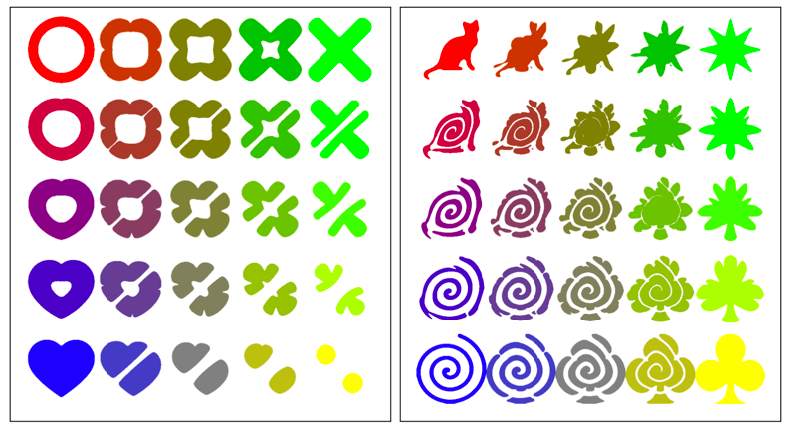
\includegraphics[scale=0.4]{wasserstein_bar.png}
\end{center}

\sect{How to compute Optimal Transport?}

\subs{Duality}

To do the computations, we embrace the setting of discrete spaces. Our
probability mesures are sum of diracs impulses:

$$ \mu = \sum_{i=1}^n a_i \delta_{x_i} \qquad \nu = \sum_{j =1}^m b_j \delta_{y_j} $$
Our cost function is a matrix $D \in \R_+^{n \times m}$ such that $D_{ij} = d(x_i, y_j)^p$. Our joint distribution $P$ is also a matrix of $\R_+^{n \times m}$ that has to satisfy several constraints that can be represented matricially. The set which $P$ belongs to is:

$$ U(a, b) = \left\{ P \in \R_+^{n \times m}~|~P \mathbbm{1}_m = a, \, P^\trans \mathbbm{1}_n = b \right\} $$

\DEF{
    The Wasserstein distance in a discrete space is defined as:
	$$ W_p^p(\mu, \nu) = \min_{P \in U(a, b)} \langle P, D \rangle $$
	\vspace{-6mm}
}

\paragraph{Dual} We now focus on the dual problem. For this we introduce the lagrangian.

$$ L(P, \alpha, \beta) = \langle P, D \rangle + \alpha^\trans (a - P \mathbbm{1}_m) + \beta^\trans (b - P^\trans \mathbbm{1}_n) $$
The objective function of the dual is:
$$ g(\alpha, \beta) = \min_{P \geqslant 0} L(P, \alpha, \beta) = \min_{P \geqslant 0} \alpha^\trans a + \beta^\trans b + \langle P, D - \alpha \mathbbm{1}_m^\trans - \mathbbm{1}_n \beta^\trans \rangle $$
If the matrix $D - \alpha \mathbbm{1}_m^\trans - \mathbbm{1}_n \beta^\trans$ has a negative coefficient, then by having this coefficient grow toward $+\infty$ we obtain a minimum of $-\infty$. But if all the coefficients are non negative, then  $\langle P, D - \alpha
\mathbbm{1}_m^\trans - \mathbbm{1}_n \beta^\trans \rangle$ is non negative and we just have to take $P=0$ to obtain a non zero value. We therefore obtain:
$$ g(\alpha, \beta) = \left\{ \begin{array}{ll}
\alpha^\trans a + \beta^\trans b & \text{si } D - \alpha \mathbbm{1}_m^\trans - \mathbbm{1}_n \beta^\trans \geqslant 0 \\
-\infty & \text{sinon}
\end{array}\right. $$

Finally, the dual problem is the maximization of this function $g$.

\DEF{
	The \textbf{dual} of the optimal transport problem is:
	$$ W_p^p(\mu, \nu) = \max_{\alpha \in \R^n, \, \beta \in \R^m \atop \alpha_i + \beta_j \leqslant D(x_i, y_j)^p} \alpha^\trans a + \beta^\trans b $$
	\vspace{-5mm}
}

Using a minimum flow solver, we can solve this linear optimization problem in
$\mathcal{O}(n^3 \log (n))$. But the solution is not stable, as illustrated
on the following figure. If we slightly move our distance $D$ or if we change
the source and destination mesures, the value of $P$ can drastically change,
since $P$ is a vertex of our simplex. One solution is to regularize the problem to fall back on a set $U_\alpha(a, b)$
strictly convex. This set is strictly contained in $U(a, b)$ and the optimal solution of this new problem won't be optimal for the initial problem, but will remain valid.
Finally, the regularization that we will describe allows to obtain an
interative algorithm of small complexity.
\begin{center}
	\begin{tikzpicture}[scale=20, >={latex}]
		\clip (0.2, -0.01) rectangle (0.51, 0.2);
		\draw[blue, thick] (0.1420, 0.1407) -- (0.5970, -0.1407);
		\draw[black, ->, thick] (0.2038, 0.1216) -- (0.2507, 0.1975);
		\fill[brown!40] (0.4503, 0.1444) -- (0.2251, 0.1444) -- (0.3695, 0.0000) -- (0.4503, -0.0000);
		\fill[greenTikz!60] (0.3827, 0.0946) -- (0.3827, 0.1104) -- (0.3804, 0.1148) -- (0.3759, 0.1206) -- (0.3692, 0.1263) -- (0.3602, 0.1307) -- (0.3556, 0.1321) -- (0.3489, 0.1336) -- (0.3264, 0.1336) -- (0.3219, 0.1321) -- (0.3151, 0.1278) -- (0.3129, 0.1234) -- (0.3129, 0.1191) -- (0.3151, 0.1133) -- (0.3241, 0.1018) -- (0.3444, 0.0888) -- (0.3534, 0.0859) -- (0.3714, 0.0859) -- (0.3804, 0.0917);
		\node[blue] at (0.3444, 0.0888) {$\bullet$};
		\node[blue, below=2] at (0.3444, 0.0888) {$P_\alpha$};
		\node[greenTikz] at (0.3489, 0.1119) {$\bullet$};
		\node[red] at (0.3695, 0.0000) {$\bullet$};
		\node[red, above=2] at (0.3695, 0) {$P$};
		\node at (0.482, 0.08) {$U(a, b)$};
		\node at (0.413, 0.12) {$U_\alpha(a, b)$};
		\node at (0.213, 0.165) {$D$};
	\end{tikzpicture}
\end{center}

\subs{Regularization}

The regularization that we choose consist in maximizing the entropy of the
joint-probability $P$. We exhibit a new parameter $\gamma$ that controls
the regularization and we obtain the following distance:

\DEF{
	The \textbf{regularized Wasserstein distance} is defined as follows:
	$$ W_\gamma(\mu, \nu) = \min_{P \in U(a, b)} \langle P, D \rangle - \gamma H(P) $$
	\vspace{-5mm}
} 

\paragraph{Remark}
Recall that we can consider two random variables $X$ and $Y$ such that $X \sim \mu$, $Y \sim \nu$ and $X,Y \sim P$. The entropy of $P$ is maximum when $X$ and $Y$ are independant, \emph{ie.} when $P = ab^\trans$ and this maximum entropy is thus $H(\mu) + H(\nu)$. 
The regularization therefore gives a matrix whose positive values are more
distributed.

\begin{center}
	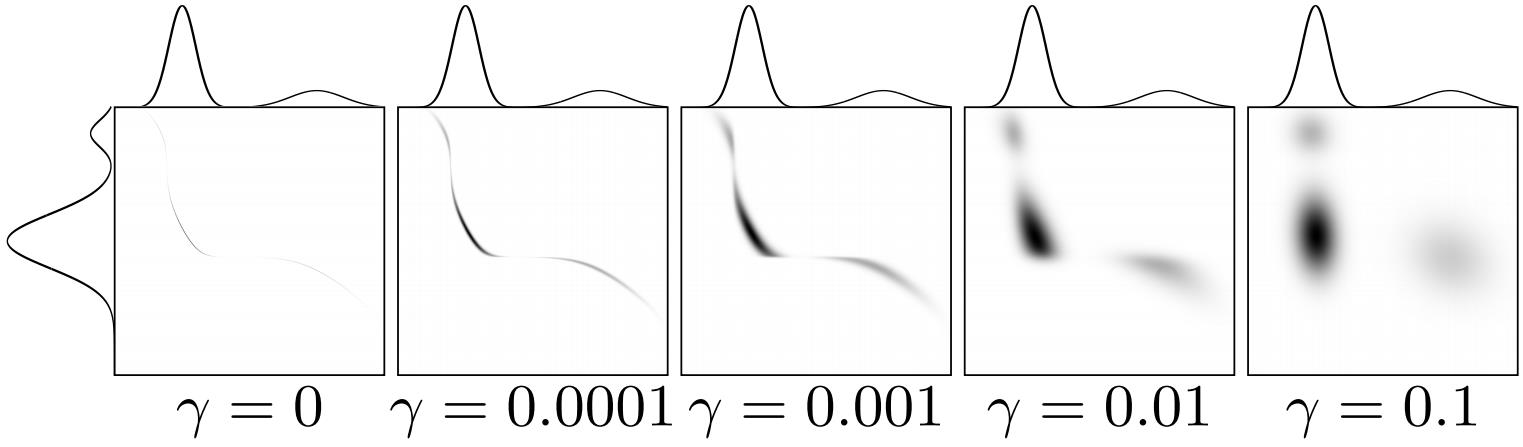
\includegraphics[scale=0.25]{reg_wass.png}
\end{center}

By strict convexity, there exist a unique matrix $P_\gamma$ that minimizes the distance:
$$ P_\gamma = \argmin_{P \in U(a, b)} \langle P, D \rangle - \gamma H(P) $$

\PROP{
    There exist a unique couple of vectors $u$ and $v$ belonging to
    $\R_+^n$ and $\R_+^m$ such that :
	$$ P_\gamma = \text{diag}(u) K \text{diag}(v), \qquad K = e^{-D / \gamma} $$
	\vspace{-6mm}
}

\dem

We write the new laplacian:

$$ L(P, \alpha, \beta) = \sum_{ij} \left( P_{ij} D_{ij} + \gamma P_{ij} \left( \log_2 P_{ij} - 1 \right) \right) + \alpha^\trans (a - P \mathbbm{1}_m) + \beta^\trans (b - P^\trans \mathbbm{1}_n) $$
We compute the partial derivative with respect to $P_{ij}$:
$$ \dfrac{\partial L}{\partial P_{ij}} = M_{ij} + \gamma \log_2 P_{ij} - \alpha_i - \beta_j $$
The dual is the maximization of the minimum of the laplacian with respect
to $P$. We must look for $P$ such that the partial derivative is equal to zero:
$$ \dfrac{\partial L}{\partial P_{ij}} = 0 \Rightarrow P_{ij} = e^{\frac{\alpha_i}{\gamma}} e^{-\frac{D_{ij}}{\gamma}}  e^{\frac{\beta_j}{\gamma}} = u_i K_{ij} v_j $$
\findem

\paragraph{Sinkhorn}
We have at our disposition an interative method to find this matrix $P_\gamma$. We use the condition $P_\gamma \in U(a,b)$:
$$ P_\gamma \in U(a, b) \Leftrightarrow \left\{ \begin{array}{lrr}
\text{diag}(u) K \text{diag}(v) \mathbbm{1}_m & = & a \\
\text{diag}(v) K^\trans \text{diag}(u) \mathbbm{1}_n & = & b
\end{array} \right. $$
$$ P_\gamma \in U(a, b) \Leftrightarrow \left\{ \begin{array}{lrr}
\text{diag}(u) K v & = & a \\
\text{diag}(v) K^\trans u & = & b
\end{array} \right. $$
Then, we introduce $\odot$ the coefficient-wise product:
$$ P_\gamma \in U(a, b) \Leftrightarrow \left\{ \begin{array}{lrr}
u \odot K v & = & a \\
v \odot K^\trans u & = & b
\end{array} \right. $$
$$ P_\gamma \in U(a, b) \Leftrightarrow \left\{ \begin{array}{lrc}
u & = & a \, / \, K v \\
v & = & b \, / \, K^\trans u
\end{array} \right. $$
Sinkhorn's algorithm is thus the following: \\
\begin{algorithm}[H]
	\caption{Sinkhorn}
	\Repeat{convergence of $u, v$}{
		$u \gets a \, / \, K v$ \;
		$v \gets b \, / \, K^\trans u$ \;
	}
\end{algorithm}

\paragraph{Complexity}
It has been proved that the algorithm converges in linear time. Moreover,
an iteration is done in $\mathcal{O}(mn)$ but the computation can be
parallelized. It is also possible to use grid convolution to obtain a
complexity of $\mathcal{O}(n \log n)$.

\paragraph{Dual}
On peut aussi relever la formulation du dual avec régularisation :
$$ W_\gamma(\mu, \nu) = \max_{\alpha, \beta} \alpha^\trans a + \beta^\trans b - \gamma \left( e^{\alpha / \gamma} \right)^\trans K \left( e^{\beta / \gamma} \right) $$

\paragraph{Lien avec la divergence KL}
We write the kernel:
$$ K_\gamma(i, j) = \exp \left( - \dfrac{d_{i, j}}{\gamma} \right) $$
We obtain a new formulation of the entropic regularization with the KL-divergence:
$$ W_\gamma(\mu, \nu) = \min_{P \in U(a, b)} \gamma KL(P | K_\gamma) $$

\sect{Optimal Transport and Machine Learning}

Now that we have convinced ourselves of the good mathematical foundations
of Optimal Transport, and of the fact that we can actually compute it, we
can wonder how we can put this tool to great use in the setting of machine
learning.

\subs{Compute the optimal transport of what?}

In the previous section we have seen that we have an algorithm to compute
optimal transport (Sinkhorn's algorithm), and that this algorithm can be
parallelized. We can take advantage of this fact to actually compute optimal
transport among huge databases. One of the application of this is similarity
based retrieval.

\paragraph{Color histograms}

The color-histogram of an image is a tool that characterizes the color
distribution of an image. Interestingly enough, it has been noticed that
color-histogram are good tool to describe the similarity of two images. Since
we now have at our disposal a tool to compute the distance between two
distribution probability, we can apply it for histograms (that are really not
that far from probability distribution, so much so that the algorithms and
methods that we described earlier are relevant even without any fondamental
change of setting). For a given image we can thus compute the distance between
its histogram and the histogram of images comming from a bigger database:
picking images that have the most similar histogram (in the sense of the
Wasserstein distance) will therefore allow some form of similarity based
image retrieval.

\begin{center}
	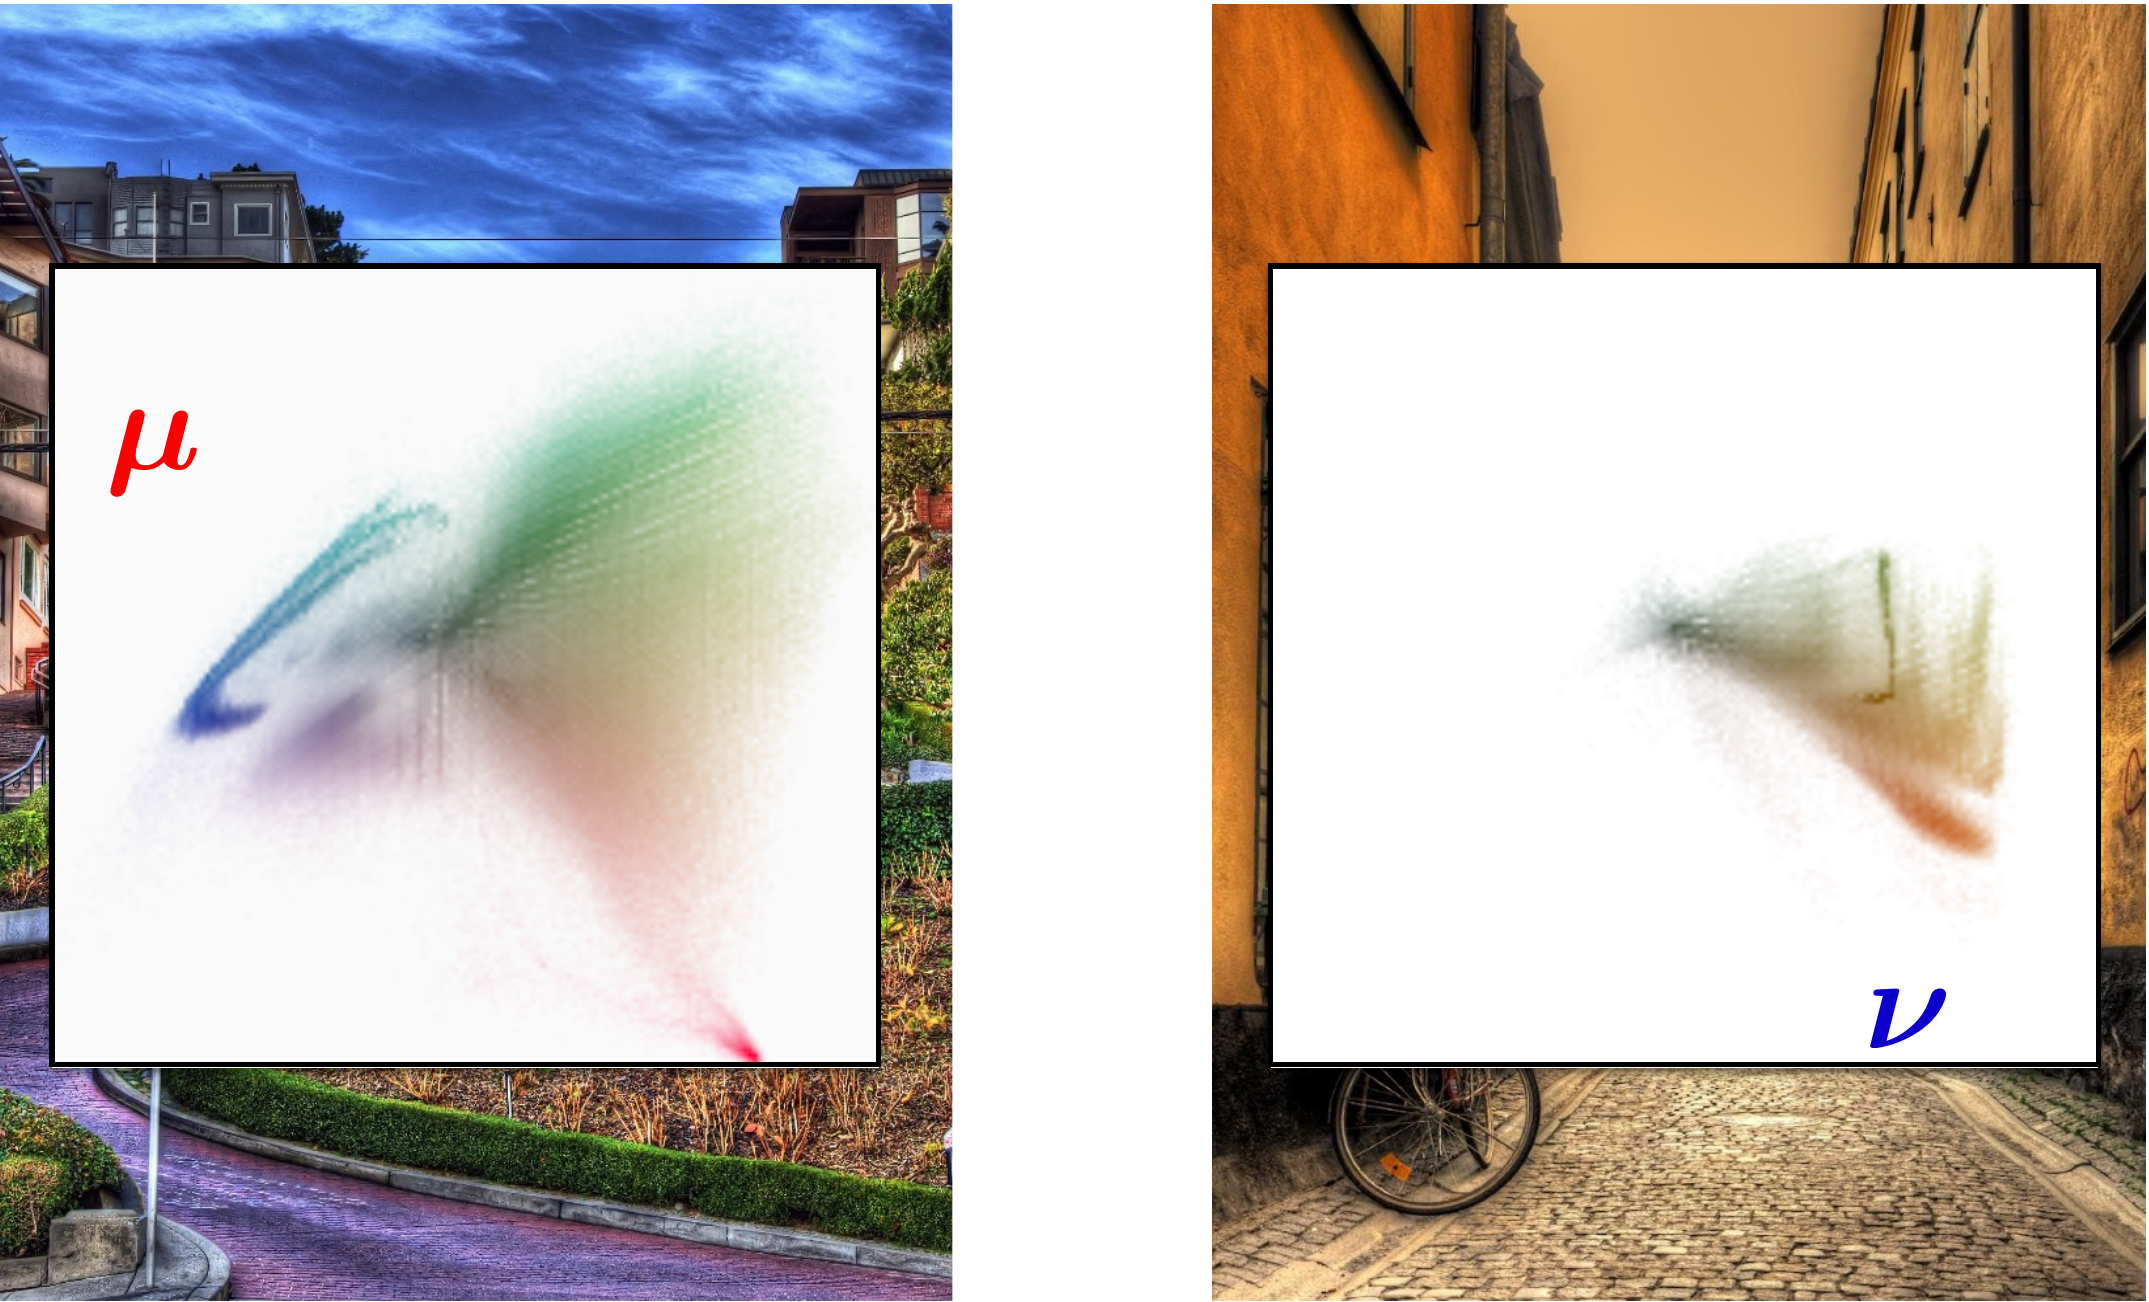
\includegraphics[scale=0.3]{image_histo.png}
    \captionof{figure}{Two images and their respective color-histograms,
    embedded in $\R^2$}
\end{center}


\paragraph{Cloud of word}

We can apply the same technique as before, but instead of considering
color-histograms, we can try to find some kind of distribution coming from
other kind of documents, for example text documents. Some previous work,
like the $\texttt{word2vec}$ framework allow for embedding of natural
language words into an Euclidean space. A text therefore defines some sort
of distribution of probability over this embedded space. As for images we
can then compare this distribution to the distributions of other texts coming
from a database (still in the sense of Wasserstein distance), and hopefully
retrieve text dealing with similar topic, although there may be some
significant differences in the actual vocabulary of those texts. We take
advantage of the geometry of the distribution of probability in the embedded
text, that tries to ensure that similar distributions are coming from texts
dealing with similar topics.

\subs{Wassersteinization}

We can go further than just using the Wasserstein to compute distance between
distributions and use this as the main tool for the machine learning problems
that we considered (we previously emphasized retrieval tasks) by introducing
the Wasserstein distance on well studied machine learning settings and
problems. We thus shed a new light on those problems, and the results are
often fruitful. Some authors have coined the term $\textbf{Wassersteinization}$
for this process.

\DEF{
	$\textbf{Wassersteinization}$ is the process of introducing optimal
	transport into an optimization or machine learning problem
} 

One way to approach this process is to introduce Wasserstein distance as a
loss or fidelity term in optimization problems. This will motivate the interest
toward the study of not only the very Wasserstein distance, but also of its
derivative. More precisely we can show that we can computationaly evaluate
the derivatives of the Wasserstein distance. Therefore we can deal with it a variety of optimization problems, including machine lerning related ones.

\paragraph{Averaging data}

We can also see optimal transport as a normalization tool for data. One of
the setting where this point of view as been proposed is the one of data
averaging. We have already discussed earlier the benefits of Wasserstein's
barycenters when compared to, say linear interpolations or $l_2$
barycenters. One can see this put in good use in the case of data acquired
through real world experiment. For instance, we can imagine a neurology
setting, where the goal is to study the reaction of the brain of a patient
to a certain precise stimulus. To do this we subjet the patient to the stimuli
several time and we aim to submit the measures of the brain activity to
a machine algorithm to study some of its features. But because of a whole
lot of data acquisition hazards (noise, imprecisions in the measures, etc),
the result will slighty differ from one experiment to another although it
concerns the same stimulus. Therefore computing the average of the brain
activity (that can easily seen to be analog to a probability distribution
on the brain space), in the sense of Wasserstein barycenters can hopefully
give access to more relevant data, without loosing the meaningful information.


\begin{center}
    \centering
	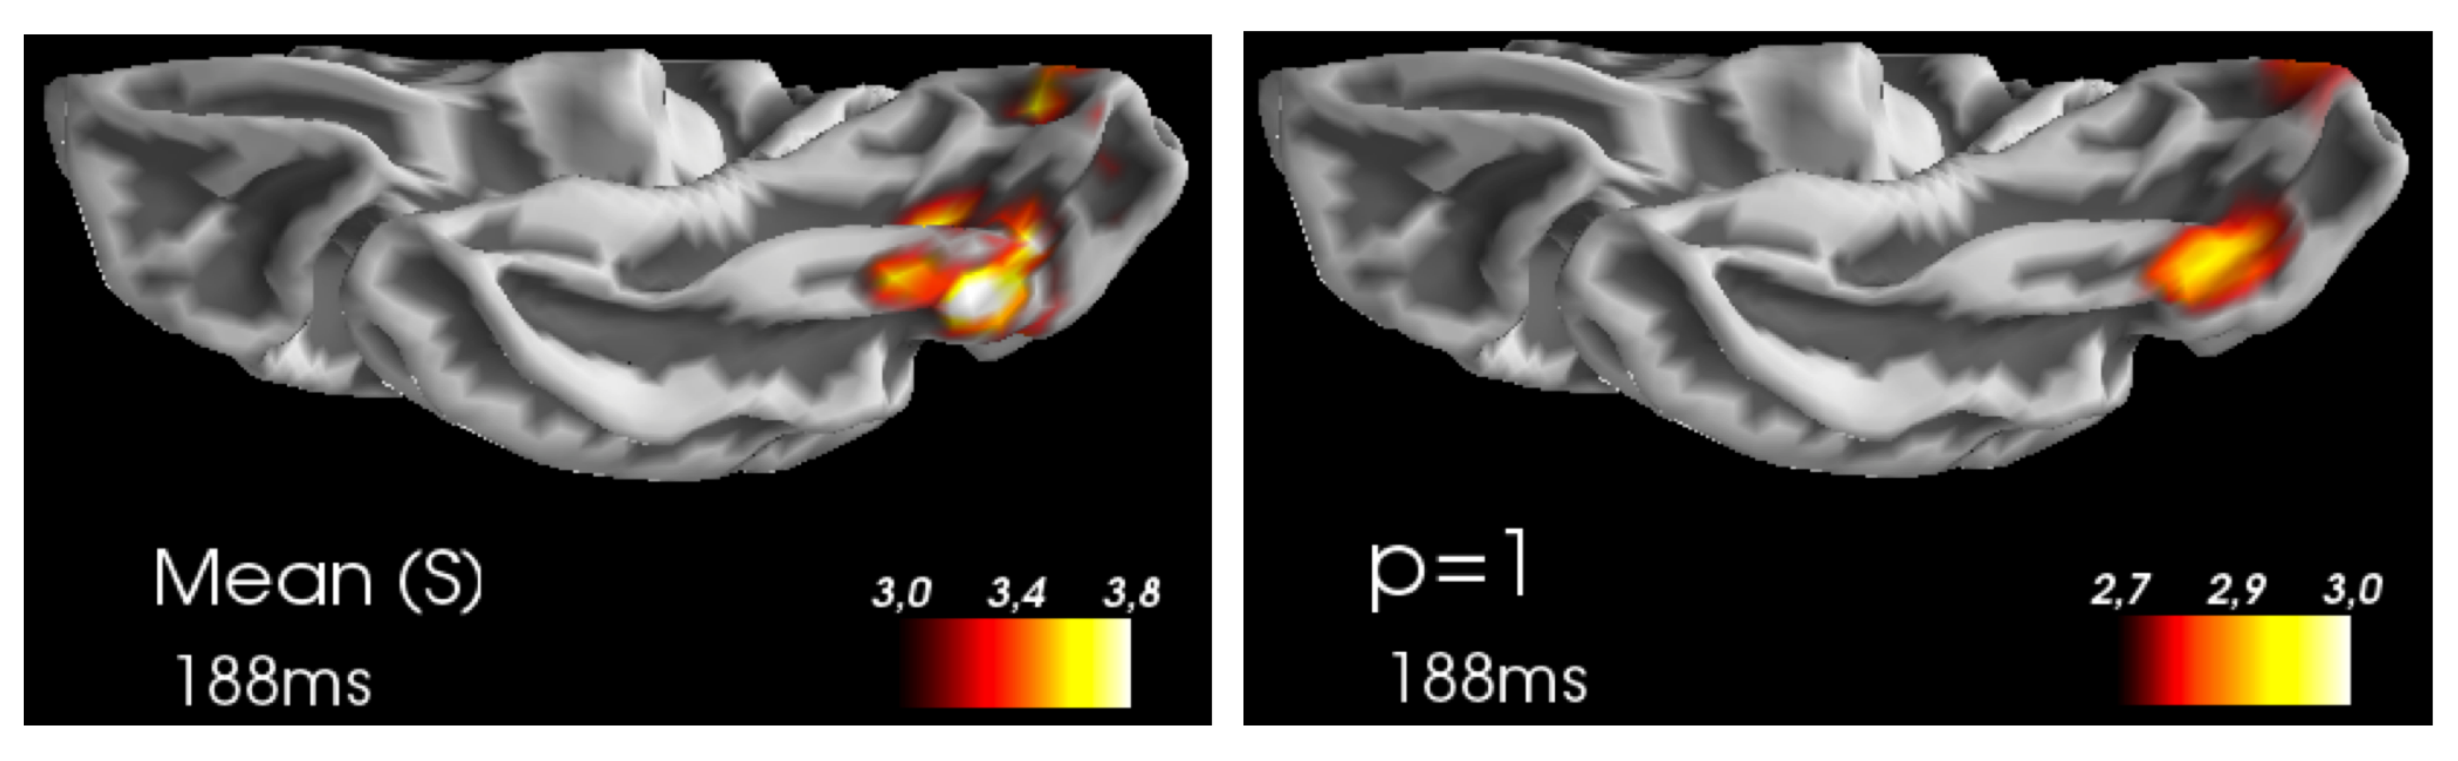
\includegraphics[scale=0.3]{brain_map.png}
    \captionof{figure}{On the left the average brain map among several
    experiments, on the right the brain activity map on a single experiment.}
\end{center}

The same idea can be followed in other fields, like imagery for instance.

\paragraph{Aggregating distributions}

Instead of processing the input of our machine learning algorithms, one can
use this idea of aggregating several distribution on the output of machine
learning algorithms. Imagine that we want to use Bayesian learning (\emph{ie.}
learn a probability distribution, in a Bayesian framework), on a dataset so
huge that it cannot even fit on a single machine, and would it fit that the
computation time would be out of control. We can imagine to split the dataset
into $J$ different parts and distribute it amongst $J$ machines running the
same learning algorithms. The result of this process is a set of $J$
distributions learned from each part of the dataset. Although they represent
the same truth, because of the variation of the data those variation will
be slightly different. Once again Wasserstein-averaging provides a useful
tool to aggregate those distributions, into an hopefully meaningful one,
closer the underlying real distribution. The good news is that this Wasserstein
posterior aggregation method comes with theoretic statistical guaranties!

%\subs{Semi-suppervised learning setting}

\paragraph{Semi-supervised learning setting}

Wasserstein propagation: smooth a graph $(V,E)$ where an histogram is associated
$\mu_v$ to each vertex $v$, with a susbset $S$ of the vertices that have a
fixed histogram (known data).

Solve the following optimization problem.

$$
    \underset{\substack{\mu_i \in \mathcal{P}\left(\Omega\right) \\ \text{for }i \in V\setminus S}}\min \sum_{(e_1, e_2) \in E} W_2^2\left(\mu_{e_1}, \mu_{e_2}\right)
$$

blabla

\paragraph{omg dictionnary learning what is this????????? :oooooo}

\subs{Wasserstein PCA, Geodesics and Inverse problem}

Since the space of distributions with the OT geometry has negative curvature,
we generalize the PCA (ie. projecting on one dimension spaces) into Generalized
Principal Geodesics. We then want to explain stuff out of what we found;
eg. affaire Bonneel vs nounours

	
	\chapter{Review of papers}

\myminitoc

\sect{Sinkhorn Distances: Lightspeed Computation of Optimal Transport \cite{Cut}}

In this paper written in 2013, Cuturi proposed one of the most currently used algorithm to compute Wasserstein distances. He smoothed the classic optimal transport problem thanks to an entropy-regularization and it leads to a new distance which has a faster solver. He also showed that using regularization gives better results on MNIST classification problem than using the classic Wasserstein distance or obviously the Euclidean distance. This paper is part of the search for adequate and easily computable distances in machine learning. Wasserstein distance is better than Euclidean distance in many cases of machine learning but because the complexity to compute it is $\mathcal{O}(n^3 \log n)$ for $n$ the size of the data Wasserstein distance is rarely used. That's why techniques to compute the Wasserstein distance had to be develop.

\paragraph{Idea}
The main ideas of this paper are the use of an entropic-regularization to simplify computation when using Sinkhorn iterative algorithm and idea of computing the distances between one point and a family of other points in the same time, to use matrix-matrix multiplications instead of matrix-vector multiplications. Thus the algorithm can be implemented on GPU architectures.

\paragraph{Regularization}
We recall that the goal of the optimal transport problem in the Kantorovich formulation is to find a joint distribution $P \in \R^{d \times d}$ where the marginals equal the two distributions for which we want to compute the distance. That is to say $P \mathbbm{1}_n = a$ and $P^\trans \mathbbm{1}_n = b$ when we compute the distance between $a$ and $b$. We call $U(a, b)$ the set of all possible values for $P$. By denoting the entropy by $H$ we can show that:
$$ H(P) \leqslant H(a) + H(b) $$
And $H(P) = H(a) + H(b)$ when $P = a b^\trans$. We then restrict $P$ to the new set:
$$ U_\alpha(a, b) = \{ P \in U(a, b) \, | \, \text{KL}(P || a b^\trans) \leqslant \alpha \} = \{ P \in U(a, b) \, | \, H(P) \geqslant H(a) + H(b) - \alpha \} $$
Two reasons are given to this restriction. The first one is that it will be easier to compute the distance. The second is that without regularization $P$ has almost $2n-1$ non-zero coefficients. The transport is almost deterministic and it is not natural. That's why smoothing the transport plan with entropic regularization is presented as a good idea. In the paper, it is shown that this restriction induce a new distance:
$$ d_{M, \alpha} = \min_{P \in U_\alpha(a, b)} \langle P, M \rangle $$
Were $M$ is a distance matrix.

\paragraph{Computation}
By duality theory he obtained that to $\alpha$, corresponds a value $\lambda \geqslant 0$ such that the distance $d_{M, \alpha}$ is equal to the distance $d_M^\lambda$ defined by:
$$ d_M^\lambda(a, b) = \langle P^\lambda, M \rangle, \quad \text{where } P^\lambda = \argmin_{P \in U(a, b)} \langle P, M \rangle - \dfrac{1}{\lambda} H(P) $$
Then Cuturi show that this new distance can be computed with a much cheaper cost than the original Wassertein distance $d_M$. In fact the iterative Sinkhorn algorithm presented below converge in few steps to the transport plan $P^\lambda$. The \figurename~\ref{recap1} summarize the relationships between all these distances.

\vspace{3mm}
\begin{algorithm}[H]
	\caption{\textsc{Sinkhorn}$\left( a, \{ b_i \}_{i=1}^N, M, \lambda \right)$}
	$B \gets \left[ b_1, \dots, b_N \right] \in \R^{n \times N}$ \;
	$K \gets \exp \left( \lambda M \right)$ \;
	$u = \left[ u_1, \dots, u_N \right] \gets \mathbbm{1}_{n \times N} \, / \, n$ \;
	\Repeat{convergence of $u$}{
		$u \gets a \, / \, \left( K \left( B \, / \, \left( K^\trans u \right) \right) \right)$ \;
	}
	$v = \left[ v_1, \dots, v_N \right] \gets B \, / \, \left( K^\trans u \right)$ \;
	$P^\lambda_i \gets \text{diag}(u_i) K \text{diag}(v_i)$ \;
	\Return $d = \left[ d_M^\lambda(a, b_1), \dots, d_M^\lambda(a, b_N) \right] = \left[ \left\langle M, P^\lambda_1 \right\rangle, \dots, \left\langle M, P^\lambda_N \right\rangle \right]$
\end{algorithm}
\vspace{3mm}

\begin{figure}
	\centering
	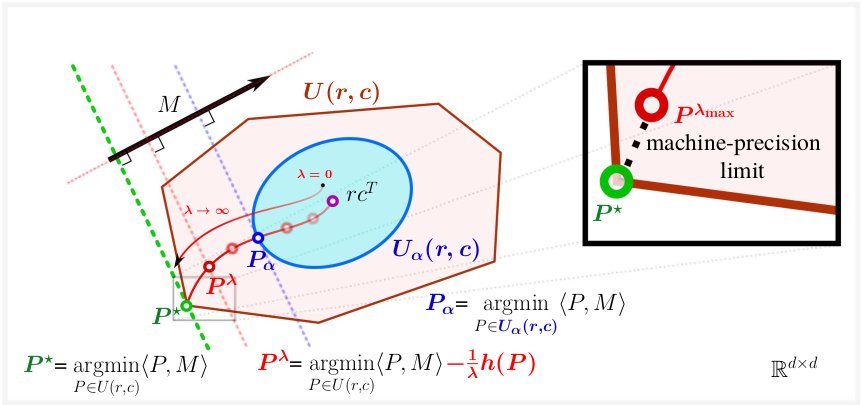
\includegraphics[scale=0.5]{recap1.png}
	\captionsetup{justification=centering}
	\caption{Graphical representation of different distances and their relationships.}
	\label{recap1}
\end{figure}

\paragraph{Results}
The regularized Wasserstein distance is then used in a SVM to classifiy images of the MNIST database. The \figurename~\ref{comp} compare the error on a test set for different distances used in the SVM. The distance EMD is the classical optimal transport. As we can see the regularized version beat all distances. Furthermore he evaluated the execution time by stopping the iterations when $\| d_{i+1} / d_i - 1 \| < 10^{-4}$ where $d_i$ is the distance obtained at the end of the iteration $i$. He gave a comparison between EMD and regularized Wasserstein for different values of $\lambda$ in the \figurename~\ref{comp2}.

\begin{figure}[h]
	\centering
	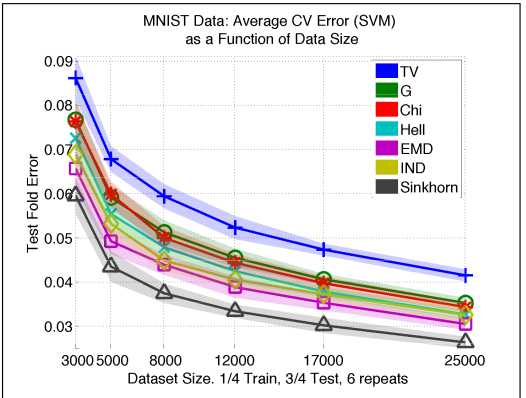
\includegraphics[scale=0.55]{comp.png}
	\caption{Test error for different distances}
	\label{comp}
\end{figure}
\begin{figure}[h]
\centering
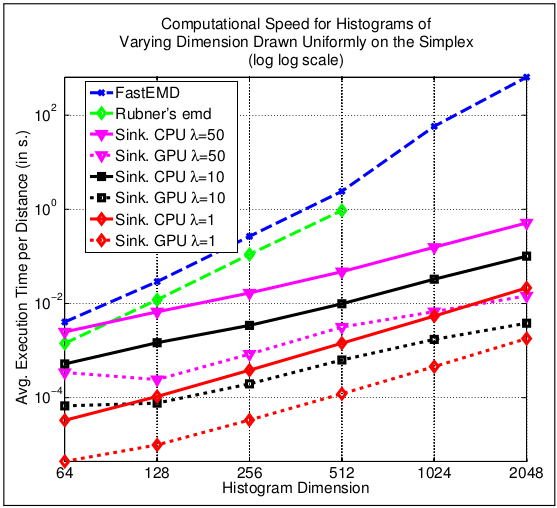
\includegraphics[scale=0.5]{comp2.png}
\caption{Execution time for different distances}
\label{comp2}
\end{figure}

\newpage

\sect{Wasserstein GAN \cite{Arj++}}

This paper proposes a new GAN training algorithm based on Wasserstein distance. When we learn a probability we need to use a divergence between probability distributions. In a first time they show the advantages of the Wasserstein distance over all well-known other divergences on probabilities. Thanks to their WGAN (for Wasserstein GAN), they cure the problem of the need of maintaining a balance between training discriminator and training generator. They also observed that the mode dropping phenomenon is reduced. Furthermore theu GAN allow to plot the Wasserstein distance continuously which is very usefull for debugging and to have an estimation of the quality.

\paragraph{Advantage of Wasserstein distance}
They illustrate the interest of Wasserstein distance on the convergence of the probability $\Pp_\theta = g_\theta(Z) = (\theta, Z)$ toward $\Pp_0 = (0, Z)$ for $Z \sim U([0, 1])$ when $\theta$ tends to 0. We have:
\begin{itemize}
	\item $W(\Pp_0, \Pp_0\theta) = | \theta |$ where $W$ is the Wasserstein distance.
	\item $JS(\Pp_0, \Pp_\theta) = \left\{ \begin{array}{ll}
			\log 2 & \text{if } \theta \neq 0 \\
			0 & \text{if } \theta = 0
		\end{array} \right.$ where $JS$ is the Jensen-Shannon divergence.
	\item $KL(\Pp_0, \Pp_\theta) = JS(\Pp_\theta, \Pp_0) = \left\{ \begin{array}{ll}
			+ \infty & \text{if } \theta \neq 0 \\
			0 & \text{if } \theta = 0
		\end{array} \right.$ where $KL$ is the Kullback-Leibler divergence.
	\item $\delta(\Pp_0, \Pp_\theta) = \left\{ \begin{array}{ll}
			1 & \text{if } \theta \neq 0 \\
			0 & \text{if } \theta = 0
		\end{array} \right.$ where $\delta$ is the total variation distance defined as $\delta(\Pp_0, \Pp_1) = \sup_{A \in \Sigma} | \Pp_0(A) - \Pp_1(A) |$ with $\Sigma$ the set of all Borel subsets.
\end{itemize}
Thus the Wasserstein distance is the only one for which there is convergence. Then a gradient descent can be applied with the Wasserstein distance but it can't with other divergences. This a just an example but they also proved the following theorem which shows the continuity under some assumptions:

\PROP{
	tada
}

\sect{Convolutional Wasserstein Distances: Efficient Optimal Transportation on Geometric Domains \cite{Goe++}}

Because a single step of Sinkhorn algorithm has a complexity in $\mathcal{O}(n^2)$, computing the Wassertein distance may take a while in many cases. That's why the researchers who write this paper thought about a more effective solution to compute a step. They found a way to use Gaussian convolution with a $\mathcal{O}(n \log n)$ complexity instead of a matrix-vector product. More generally they use a heat kernel. So instead of the convolution it can also be a sparse pre-factored linear system which can be computed in a complexity smaller than $\mathcal{O}(n^2)$. Furthermore by doing this, the convergence is still linear. Of course this can not be applied in all cases of optimal transport, but it can be used on very common geometric domains, like images or meshes. In addition of the computation of Wasserstein distance, they also propose a way to use convolution in the computation of Wasserstein barycentres and Wasserstein propagation.

\paragraph{Using a heat kernel in the entropy-regularization}
We recall what is the entropy-regularized Wasserstein distance between $\mu_0$ and $\mu_1$ on the domain $M$:
$$ W_{2, \gamma}^2(\mu_0, \mu_1) = \inf_{\pi \in \Pi} \left[ \int \int_{M \times M} d(x, y)^2 \pi(x, y) dx dy \, - \, \gamma H(\pi) \right] = \gamma \left[ 1 + \min_{\pi \in \Pi} \text{KL}(\pi | \mathcal{K}_\gamma) \right]$$
Where:
$$ \Pi = \left\{ \pi \in \text{Prob}(M \times M) \, | \, \pi(\cdot, M) = \mu_0, \pi(M, \cdot) = \mu_1 \right\} $$
$$ H(\pi) = - \int \int_{M \times M} \pi(x, y) \ln \pi(x, y) dx dy $$
$$ \mathcal{K}_\gamma = e^{-d(x, y)^2 / \gamma} $$
$$ \text{KL}(\pi | \mathcal{K}) = \int \int_{M \times M} \pi(x, y) \left[ \ln \dfrac{\pi(x, y)}{\mathcal{K}(x, y)} - 1 \right]\ln  dx dy $$
This is a strictly convex problem thanks to the entropy. The idea of the paper is to use heat kernel because is some cases, the solution of the diffusion equation can be computed in a effective way. We denote by $\mathcal{H}_t(x, y)$ the diffusion between $x$ and $y$ after a time $t$ in the heat kernel. We have:
$$ \mathcal{K}_\gamma \approx \mathcal{H}_{\gamma / 2}(x, y) $$
We won't store $\mathcal{H}$ because it has a space complexity in $\mathcal{O}(n^2)$ and we want a lower complexity. But we generally know a way to apply $\mathcal{H}$ to a vector. In the case of images we apply Gaussian convolution with $\sigma^2 = \gamma$. \\
In the case of triangle meshes we associate a weight to faces proportional to their area. We denote by $a$ the vector of these weights (In images of size $n \times m$ we set $a = 1 / (nm)$). Then we denote by $L$ the cotangent Laplacian and by $D_a$ the diagonal matrix with diagonal $a$. By discretizing the heat equation, we obtain:
$$ w = \mathcal{H}_t(v) \Leftrightarrow \left( D_a + t L \right) w = v $$
The linear system can be solved efficiently by pre-computing a sparse Cholesky factorization.

\paragraph{Algorithm}
We some computations we arrive at:

\vspace{3mm}
\begin{algorithm}[H]
	\caption{\textsc{Convolutional-Sinkhorn}($\mu_0, \mu_1, H_t, a$)}
	$v, w \gets 1$ \;
	\Repeat{convergence of $v, w$}{
		$v \gets \mu_0 \oslash H_t(a \otimes w)$ \;
		$w \gets \mu_1 \oslash H_t(a \otimes v)$ \;
	}
	\Return $2t a^\trans \left[ \left( \mu_0 \otimes \ln v \right) + \left( \mu_1 \otimes \ln w \right) \right]$
\end{algorithm}
\vspace{3mm}

Where $\oslash$ and $\otimes$ denote element-wise operations. As Sinkhorn algorithm we obtain a simple iterative algorithm where, this time, steps can be computed in $\mathcal{O}(n \log n)$ in many cases, where $n$ is the size of the domain $M$.

\paragraph{Barycenter}
An algorithm for computing barycenters is also provided. We won't enter into details but we give their algorithm for computing the barycenter of distributions $\mu_i$ associated with weights $\alpha_i$ for $1 \leqslant i \leqslant k$:

\vspace{3mm}
\begin{algorithm}[H]
	\caption{\textsc{Convolutional-Barycenter}($\{\mu_i\}, \{ \alpha_i \}, H_t, a$)}
	$v_1, \dots, v_k \gets 1$ \;
	$w_1, \dots, w_k \gets 1$ \;
	\Repeat{convergence of $v_i, w_i$}{
		$\mu \gets 1$ \;
		\For{$i = 1, \dots, k$}{
			$w_i \gets \mu_i \oslash H_t(a \otimes v_i)$ \;
			$d_i \gets v_i \otimes H_t(a \otimes w_i)$ \;
			$\mu \gets \mu \otimes d_i^{\alpha_i}$ \;
		}
		\vspace{3mm}
		// Optional \;
		$\mu \gets $ \textsc{Entropic-Sharpening}$\left( \mu, \max_i H(\mu_i) \right)$ \;
		\vspace{3mm}
		\For{$i = 1, \dots, k$}{
			$v_i \gets v_i \otimes \mu \oslash d_i$ \;
		}
	}
	\Return $2t a^\trans \left[ \left( \mu_0 \otimes \ln v \right) + \left( \mu_1 \otimes \ln w \right) \right]$
\end{algorithm}
\vspace{3mm}
Where entropic sharpening allow us to make the entropy of the result $\mu$ smaller than the maximum entropy of all $\mu_i$. To do so if $H(\mu)$ is greater than $\max_i H(\mu_i)$, then we set $\mu$ to $\mu^\beta$ where $\beta$ is such that $H(\mu^\beta) = \max_i H(\mu_i)$. We can find $\beta$ using Newton's method.

\paragraph{Applications}
This has many applications in geometric domains. Applications that are given are:
\begin{itemize}
	\item Shape interpolation (\figurename~\ref{shape})
		\begin{figure}[h]
			\centering
			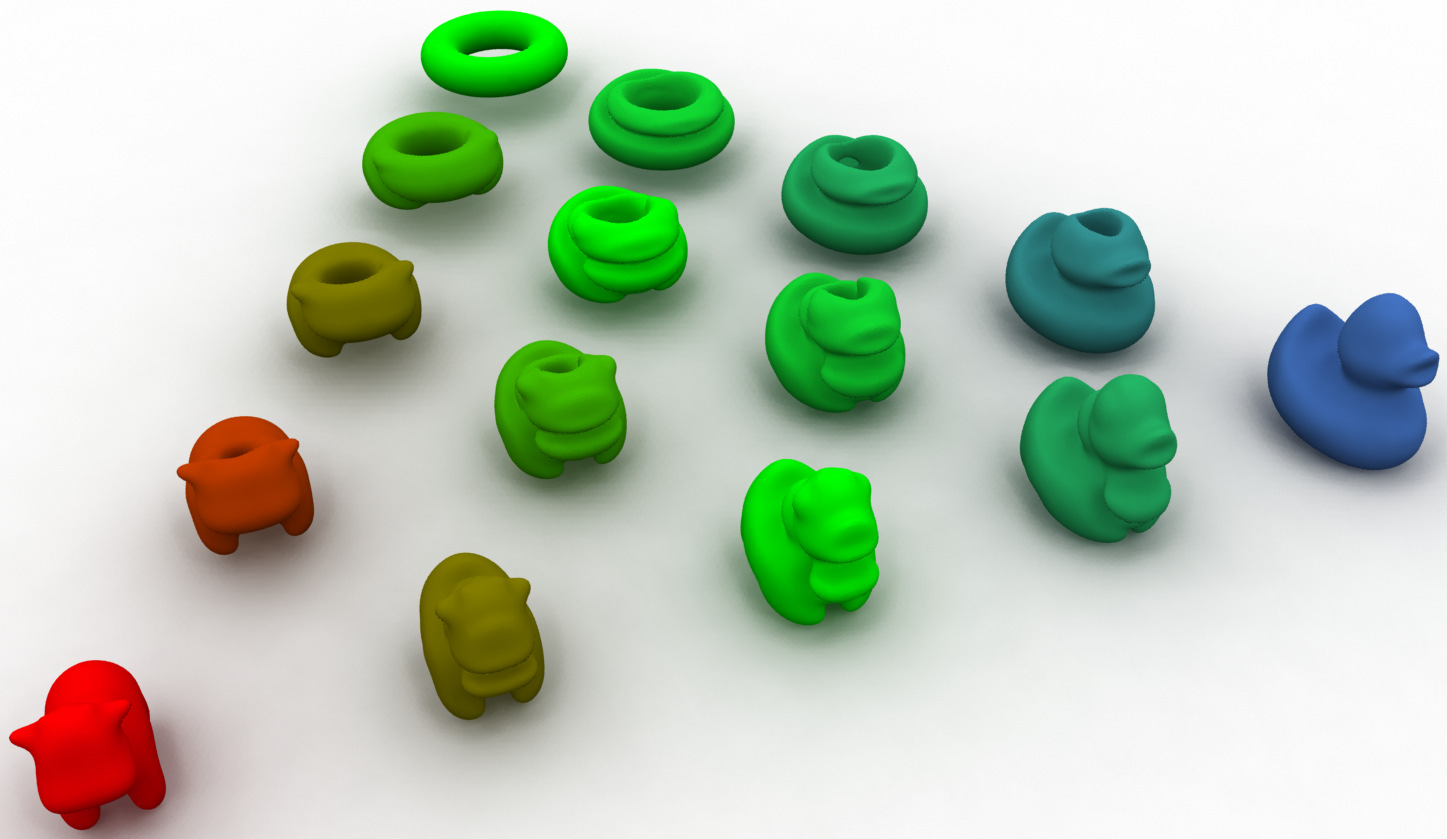
\includegraphics[scale=0.22]{shape_int.png}
			\caption{Application to shape interpolation}
			\label{shape}
		\end{figure}
	\item BRDF design
	\item Color histogram manipulation
	\item Skeleton layout
	\item Soft maps
\end{itemize}
Finally \figurename~\ref{barp} and \figurename~\ref{cardp} are two images of barycenters they have computed. The first one is an image where we find barycenters of four images that are in the corners. The second is an interpolation between two cards. As we tried to reproduce it in the implementation part we put them here:

\begin{figure}[h]
	\centering
	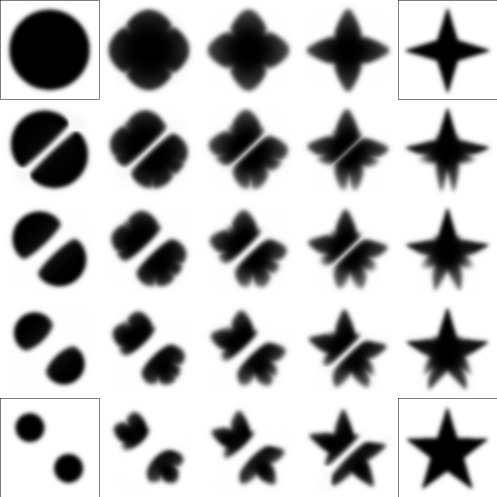
\includegraphics[scale=0.28]{bars_paper.png}
	\caption{Barycenters of four images}
	\label{barp}
\end{figure}
\begin{figure}[h]
	\centering
	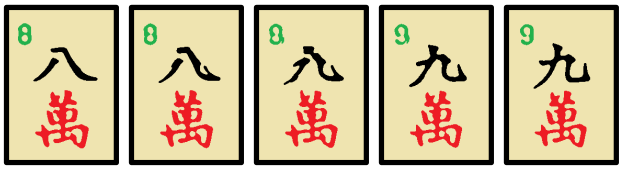
\includegraphics[scale=0.45]{cards_paper.png}
	\caption{Interpolation of two images of cards for times $t = 0, 0.25, 0.5, 0.75, 1$.}
	\label{cardp}
\end{figure}

	\chapter{Implementation}

We decided to implement the last paper to compute Wasserstein distances on images in a efficient way. We then use convolutional Sinkhorn in SVM as Marco Cuturi used Sinkhorn in his paper to classify images of the MNIST digit database \cite{Cut}. The implementation of the convolutional Wassertein distance has been written in C++. We then write the Gramm matrix of a subset of the MNIST database in a file and use it in a Python script to use SVM from Sklearn library.

\paragraph{How to use our code}
OpenMP has been used to parallelize the code. If you don't have OpenMP already install, you can install it with \verb|sudo apt install libomp-dev|.
To compile the C++ code you just have to type \verb|make|. Then you need to obtain the train image datatset and the train label dataset of the MNIST database \url{http://yann.lecun.com/exdb/mnist/}. To do so you have to run the script \verb|get_mnist.sh| which will download and rename the files correctly. The executable \verb|main| created by \verb|make| command can be used in four ways.
\begin{itemize}
	\item  \verb|./main bar| to reproduce an image similar to the \figurename~\ref{barp}; An image containing different barycenters of four shapes.
	\item \verb|./main card| to reproduce images similar to the \figurename~\ref{cardp}; An interpolation of two images of cards.
	\item \verb|./main wass > kernel.txt| to compute a kernel with the convolutional Wasserstein distance of \verb|N_TRAIN| images of the MNIST dataset. We project \verb|N_TEST| other digit images of the MNIST dataset on the kernel space created. You can change the parameter \verb|N_TRAIN| and \verb|N_TEST| at the beginning of the file \verb|src/main.cpp|. The kernel will then be written if the file \verb|kernel.txt|.
	\item \verb|./main eucl > kernel.txt| to do the same as the previous command but with Euclidean distance instead of Wasserstein distance. 
\end{itemize}
Finally when a kernel file is computed you can test SVM on it thanks to the python script \verb|learning.py|. Because computing Wasserstein kernel may take a while we provide the Wasserstein kernel \verb|kernels/wass.txt| and the Euclidean kernel \verb|kernels/eucl.txt|. You can then run:
\begin{center}
	\verb=python3 learning.py < [kernels/wass.txt | kernels/eucl.txt]=
\end{center}
It will print the performances of these two kernels, show the projection of the data on the two principle components and finally show the kernel matrix.

\paragraph{Barycenters}
We first computed some barycenters to be sure that everything works. The code for computing Wasserstein distances and barycenters is in the file \verb|src/wasserstein.cpp|. The code that produce the barycenters that we will present is in the file \verb|examples.cpp|. The first example is the reproduction of \figurename~\ref{barp}. Here is what we obtained:

\begin{figure}[h]
	\centering
	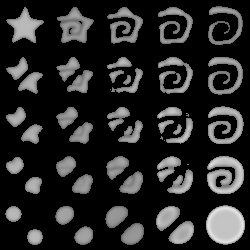
\includegraphics[scale=0.5]{bars_own.png}
	\caption{Reproduction of \figurename~\ref{barp}}
\end{figure}

The result seems to be correct. We then try on larger images, the card images that we can find in the original paper presenting convolutional Wassertein \cite{Goe++}. Here is what we obtained:

\begin{figure}[h]
	\centering
	\begin{tikzpicture}
		\node[] at (0, 0) {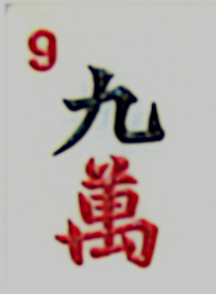
\includegraphics[scale=0.3]{bar0.png}};
		\node[] at (2.8, 0) {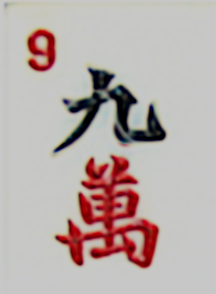
\includegraphics[scale=0.3]{bar3.png}};
		\node[] at (5.6, 0) {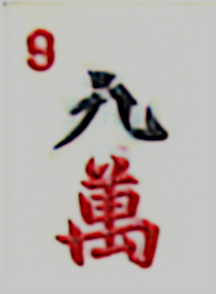
\includegraphics[scale=0.3]{bar6.png}};
		\node[] at (8.4, 0) {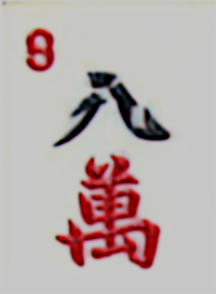
\includegraphics[scale=0.3]{bar8.png}};
		\node[] at (11.2, 0) {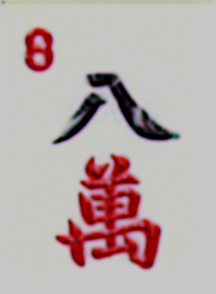
\includegraphics[scale=0.3]{bar11.png}};
		\node[] at (14, 0) {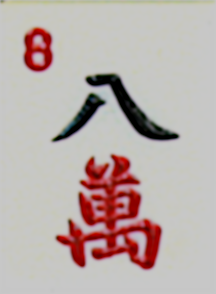
\includegraphics[scale=0.3]{bar14.png}};
	\end{tikzpicture}
	\caption{Reproduction of \figurename~\ref{cardp}}
\end{figure}

\paragraph{SVM usage}
As proposed in the paper of Cuturi \cite{Cut}, we used the Wasserstein distance to compute the Gram matrix for 500 image and we used it as a kernel in a SVM. On a test set of 1500 images we obtained 92.4\% of good answers. Whereas with a kernel using Euclidean distance we obtain a good answer on only 88.4\%. To check these results you can run the python script \verb|learning.py| on the two kernels that are in the \verb|kernels| folder.
		
	\newpage
	\appendix
	
	\bibliographystyle{alpha}
	\bibliography{bib.bib}
	
\end{document}
